\documentclass[journal]{IEEEtran}
\usepackage{amsmath,amsfonts,amssymb}
\usepackage{array}
\usepackage{textcomp}
\usepackage{stfloats}
\usepackage{url}
\usepackage{verbatim}
\usepackage{graphicx}
\usepackage[caption=false,font=footnotesize]{subfig}
\usepackage{tabularx}
\usepackage{gensymb}  
\usepackage{enumitem}
\usepackage{booktabs}
\usepackage{algorithm}
\usepackage{algpseudocode}  
\usepackage{xfrac}
\usepackage[colorlinks=true, linkcolor=blue, citecolor=blue, urlcolor=blue]{hyperref}
\usepackage{cite}
\usepackage{xcolor}
\usepackage{soul}

\begin{document}
\bstctlcite{IEEEexample:BSTcontrol}


\title{Integrated Sensing and Communication with a Single Steerable VCSEL: Fundamental Limits of RSS-Based Direction Finding}
% Alternativas:
%\title{Joint Steering and Divergence Control for VCSEL Beam Acquisition and Communication}
% \title{Sense, Then Serve: CRLB-Driven Beam Acquisition for Steerable VCSEL-Based Optical Wireless Communication}
% \title{One Beam to Find and Serve: Direction Finding and Beam Alignment with a Steerable, Divergence-Controllable VCSEL}


\author{To be determinate
\thanks{Manuscript received MM DD, 2025.
This work was supported in part by the French National Research Agency (ANR) through the Project SAFELiFi under Grant ANR-21-CE25-0001-01, and in part by the European Union's Smart Networks and Services Joint Undertaking (SNS JU) under grant agreement No. 101139292 (\textit{Corresponding author: Kevin Acuna-Condori.})
}
\thanks{
The authors are with the Université Paris-Saclay, UVSQ, LISV, 78140, Vélizy-Villacoublay, France (e-mail: kevin-jose.acuna-condori@uvsq.fr).
}
}
\markboth{IEEE Transactions on Communications,~Vol.~XX, No.~X, 2026}%
{Acuna-Condori \MakeLowercase{\textit{et al.}}: Model-Based Beam-Steered OWP with Single-LED Single-PD for 3D Localization}
\maketitle

\begin{abstract}
Narrow-beam optical wireless communication (OWC) links based on
vertical-cavity surface-emitting lasers (VCSELs) can deliver very high
data rates, but only if the transmitter knows where to point. We propose
an integrated sensing and communication (ISAC) scheme in which a single
steerable VCSEL, with controllable orientation and divergence, first
senses the direction of the user equipment (UE) and then uses the same
beam to serve it. The transmitter probes the room with a few wide beams,
refines the estimate with narrower ones, and finally points a narrow beam
at the UE, relying only on the received signal strength (RSS) reported by
a single photodiode. We derive the Cram\'er--Rao lower bound for this
direction-finding problem and use it to design the probing beams, jointly
selecting their orientations and divergences to balance sensing time,
pointing accuracy, and the throughput of the subsequent link.
% TODO: añadir una frase con el resultado principal cuando esté disponible.
\end{abstract}


\begin{IEEEkeywords} 
    3D indoor localization, beam steering, Cramér-Rao bounds, optical wireless communications, optical wireless positioning
\end{IEEEkeywords}


% =====================================================================
\section{Introduction}
% =====================================================================

The rapid growth of wireless data traffic is expected to push the
radio-frequency (RF) spectrum toward a capacity crunch in the coming
years~\cite{TODO_spectrum_crunch}. Providing additional spectral resources
is therefore among the objectives of sixth-generation (6G)
systems~\cite{Trevlakis2023}, and optical wireless communication (OWC) has
emerged as a promising candidate technology owing to its vast, unlicensed
spectrum~\cite{Kahn1997}.

An OWC link consists of a light source and an optical receiver, typically
a photodiode (PD), and has shown strong potential not only for
communication but also for sensing and
positioning~\cite{Zhu2025,Wang2024b}. Most OWC systems rely on
light-emitting diodes (LEDs). Despite advantages such as inherent
physical-layer security, since light is confined by opaque walls,
LED-based systems are limited by the modulation bandwidth of LEDs:
although laboratory demonstrations have reached a few Gb/s, practical
systems typically deliver data rates comparable to those of
Wi-Fi~\cite{Haas:16}, which may fall short of 6G requirements.

Laser diodes (LDs), and in particular vertical-cavity surface-emitting
lasers (VCSELs), have therefore attracted growing interest, as they enable
experimental data rates ranging from several Gb/s up to the Tb/s
regime~\cite{Hu2024,Sarbazi2020,Kazemi_GoB}. This performance comes at a price: owing
to their narrow beams, LD-based links are highly sensitive to
misalignment, and the transmitter must point accurately at the user
equipment (UE) to operate optimally. Knowing where to point is thus
a prerequisite for any high-speed LD-based link.

Several approaches have been proposed to address this problem. Kazemi
\emph{et al.}~\cite{Kazemi_GoB} proposed a grid-of-beams (GoB) transmitter
composed of a $5\times5$ VCSEL array followed by a fixed lens to extend
coverage, although its use for beam steering was not explored. The same
concept was later applied to beam steering by switching among the
elements of a $4\times4$ VCSEL array to select the beam directed toward
the user~\cite{Muller2025,Muller2026}; this architecture, however, lacks
flexibility, since the divergence cannot be controlled and the coverage is
restricted by the fixed lens. Safi \emph{et al.}~\cite{Safi_VarDiv}
showed that adding variable divergence to a GoB transmitter improves
coverage, while Ahmad \emph{et al.}~\cite{Rizwana_GoB} demonstrated that
the PD pose can be estimated with machine learning (ML) using a $5\times5$
GoB with a fixed lens. More recently, Dong \emph{et al.}~\cite{Dong_Scan}
proposed a LiDAR-inspired approach in which a single VCSEL, mounted on a
2D rotating platform covering $360^\circ$ in azimuth and $90^\circ$ in
elevation, scans the entire room to estimate the PD pose; this solution,
however, requires an extensive angular acquisition of about
$32.4\times10^{3}$ received signal strength (RSS) measurements to locate a
single UE. Collectively, these works highlight the importance of knowing
the UE location to steer the beam, maximize the signal-to-noise ratio
(SNR), and maintain line-of-sight (LoS) alignment. They also expose the
limitations of current acquisition schemes: fixed-lens GoB transmitters
offer a discrete set of beams whose coverage and resolution are fixed by
the hardware, data-driven estimators must be trained for a specific
array, and exhaustive mechanical scanning is slow and relies on moving
parts.

In parallel, non-mechanical beam-steering systems have matured. Kacker
\emph{et al.}~\cite{Kacker_3lens} presented a three-lens beam-steering
design for satellite optical communication over distances of
30--175\,km, focusing on the optical design, and the MOSAIC
project~\cite{MOSAIC} studied the optics of this approach more generally,
showing that the beam direction can be controlled with liquid lenses
while a third lens controls the divergence. These works address
how to steer the beam, but they assume that the target direction
is known or provided by an auxiliary system.

These two lines of research have so far evolved separately, and this
paper addresses the gap between them. Acquisition schemes estimate the UE
location but rely on fixed beams, training data, or exhaustive mechanical
scanning, whereas non-mechanical beam-steering systems offer flexible
control of direction and divergence but do not address how to find the
receiver. A transmitter with such control is, however, not only a
communication device but also a sensing instrument: by probing the room
with a few beams and collecting the RSS at the UE, it can estimate the UE
direction and then reuse the same beam, narrowed, to deliver data. This
enables integrated sensing and communication (ISAC) with a single device,
without additional sensors, positioning infrastructure, or training data.
Realizing this concept raises questions that the literature has not yet
answered. How accurately can the UE direction be estimated from RSS
measurements of a steerable, divergence-controllable beam? How many
probing beams are needed, and with which orientations and divergences?
And how does the time spent on sensing trade off against pointing
accuracy and, ultimately, against the throughput of the subsequent
communication link?

To answer these questions, we consider a single steerable single-mode
VCSEL whose beam direction and divergence are treated as control
parameters, abstracting the specific optical implementation. Rather than
estimating the full 3D position of the UE, we focus on its direction,
which is the quantity required to point the transmitter. The main
contributions of this paper are as follows:
\begin{itemize}
  \item A single-device ISAC framework in which a steerable VCSEL with
  controllable orientation and divergence estimates the UE direction
  from RSS feedback, through a wide-beam scan and a local refinement,
  and then reuses the same beam, narrowed, for data transmission.
  \item A closed-form Cram\'er--Rao lower bound (CRLB) for RSS-based
  direction finding with unknown range. In the far field, the bound
  factorizes into a scalar radiometric term and a geometric matrix that
  depends only on the probing beams, which makes direction finding
  calibration-free. We also establish the identifiability condition and
  the validity domain of the far-field bound.
  \item A CRLB-driven design of the scan and refinement beam sets that
  quantifies the trade-off between the number of probing beams, i.e.,
  the sensing time, and the pointing accuracy, together with a
  maximum-likelihood estimator that asymptotically attains the bound.
  % Contribución reservada para la etapa de comunicación (Hossein):
  \item An end-to-end evaluation that links the direction-estimation
  error and the sensing overhead to the SNR, achievable rate, and
  effective throughput of the narrow-beam OWC link.
\end{itemize}

% Ajustar a la estructura final del paper:
The remainder of this paper is organized as follows.
Section~\ref{sec:system} describes the system model and the operating
principle. Section~\ref{sec:crlb} derives the CRLB for direction finding.
Section~\ref{sec:design} addresses the design of the scan and refinement
stages, and Section~\ref{sec:comm} analyzes the communication stage.
Numerical results are presented in Section~\ref{sec:results}, and
Section~\ref{sec:conclusion} concludes the paper.

% =====================================================================
\section{System Model and Operating Principle}\label{sec:system}
% =====================================================================

\begin{figure}[t]
  \centering
  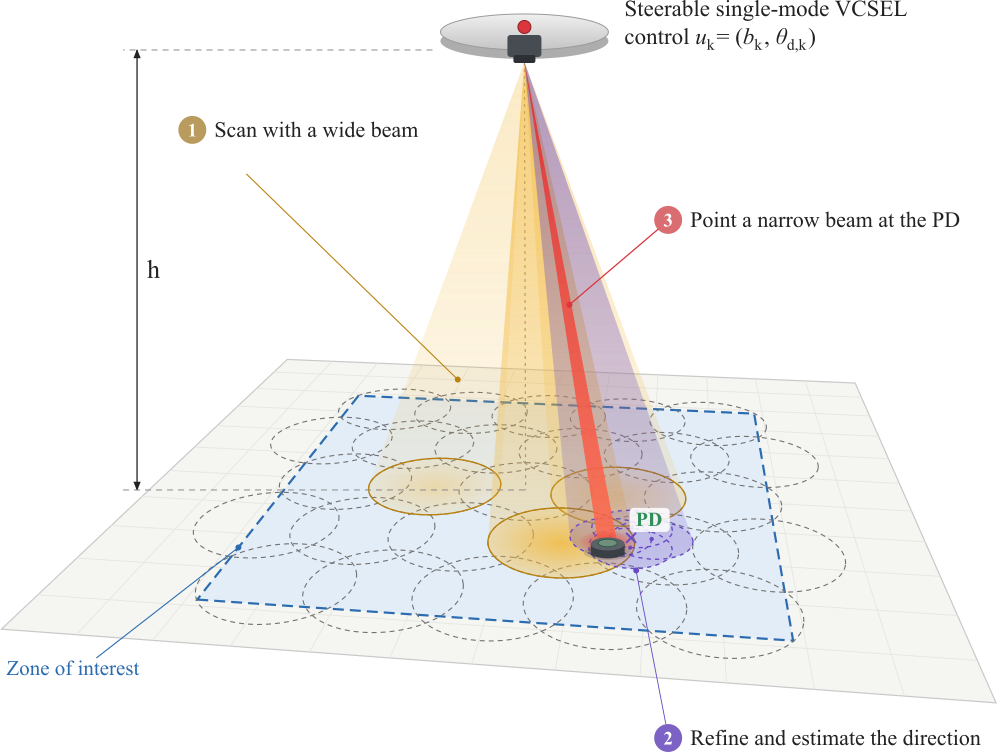
\includegraphics[width=\columnwidth]{Figures/owp_beam_steering_concept.png}
  \caption{Proposed ISAC scheme with a single steerable VCSEL:
  (1)~coarse scan with wide beams, (2)~local refinement around the coarse
  estimate, and (3)~pointing of a narrow beam at the PD for data
  transmission.}
  \label{fig:concept}
\end{figure}

\subsection{Geometry and Beam Control}

We consider an indoor room of size $L\times W\times H$. The transmitter is
a steerable single-mode VCSEL located at the center of the ceiling, which
is taken as the origin of the coordinate system, with the $z$-axis
pointing upward and the boresight along $-z$. The UE carries a single PD
that can move freely within a zone of interest $\mathcal{A}$ of size
$L_{\mathcal{A}}\times W_{\mathcal{A}}\times h_{\max}$, where $h_{\max}$
is the maximum receiver height above the floor. The PD normal is tilted
by an angle $\theta_{\mathrm{PD}}$ with respect to the $z$-axis, with
azimuth $\omega_{\mathrm{PD}}$, i.e.,
$\mathbf{n}=[\sin\theta_{\mathrm{PD}}\cos\omega_{\mathrm{PD}},\
\sin\theta_{\mathrm{PD}}\sin\omega_{\mathrm{PD}},\
\cos\theta_{\mathrm{PD}}]^{\top}$.

The beam-steering system is abstracted by the control vector
$\mathbf{c}_k=[\alpha_{x,k},\alpha_{y,k},\theta_{\mathrm{d},k}]^{\top}$
of the $k$-th beam, where $\alpha_{x,k}$ and $\alpha_{y,k}$ set the beam
orientation and $\theta_{\mathrm{d},k}$ its divergence (half-angle at
$1/e^{2}$). The controls are confined to
$\alpha_{x}\in[\alpha_{x}^{\min},\alpha_{x}^{\max}]$,
$\alpha_{y}\in[\alpha_{y}^{\min},\alpha_{y}^{\max}]$, and
$\theta_{\mathrm{d}}\in[\theta_{\mathrm{d}}^{\min},\theta_{\mathrm{d}}^{\max}]$.
The beam axis is
\begin{equation}
  \mathbf{b}(\alpha_x,\alpha_y)=
  \frac{[\tan\alpha_x,\ \tan\alpha_y,\ -1]^{\top}}
       {\sqrt{1+\tan^{2}\alpha_x+\tan^{2}\alpha_y}},
  \label{eq:beam_axis}
\end{equation}
where $\alpha_x$ ($\alpha_y$) is the angle between the $-z$-axis and the
projection of the beam axis onto the $xz$ ($yz$) plane. This
parametrization is consistent with the deflection produced by decentered
variable-focus lenses~\cite{MOSAIC}, and a uniform grid in
$(\tan\alpha_x,\tan\alpha_y)$ maps onto a uniform grid of beam centers on
any horizontal plane. We assume ideal steering: the beam remains a
circular Gaussian beam rotated rigidly about the origin, without
steering-dependent losses, and the coupling between steering and
divergence inherent to lens-based implementations is compensated by the
feedforward controller of the steering optics. The optical power
$P_{\mathrm{opt}}$ is the same for all divergences.

The UE direction is described by the unit vector
$\mathbf{u}=\mathbf{b}(\alpha_x^{\star},\alpha_y^{\star})$, where
$\boldsymbol{\alpha}^{\star}=[\alpha_x^{\star},\alpha_y^{\star}]^{\top}$
are the steering angles that point the beam at the UE. The UE position is
$\mathbf{p}=d\,\mathbf{u}$, where $d$ is the unknown range.

\subsection{Channel and Measurement Model}

The output of the single-mode VCSEL is modeled as a Gaussian
beam~\cite{Saleh2019}. For the $k$-th beam, with axis
$\mathbf{b}_k=\mathbf{b}(\alpha_{x,k},\alpha_{y,k})$, let $\phi_k$ denote
the angle between the beam axis and the UE direction, so that
$\cos\phi_k=\mathbf{b}_k^{\top}\mathbf{u}$. The intensity at the PD is
\begin{equation}
  I_k=\frac{2P_{\mathrm{opt}}}{\pi w_k^{2}(d\cos\phi_k)}
  \exp\!\left(-\frac{2d^{2}\sin^{2}\phi_k}{w_k^{2}(d\cos\phi_k)}\right),
  \label{eq:intensity}
\end{equation}
where $w_k(z)=w_{0,k}\sqrt{1+(z/z_{R,k})^{2}}$ is the beam radius, with
waist $w_{0,k}=\lambda/(\pi\theta_{\mathrm{d},k})$ and Rayleigh range
$z_{R,k}=\pi w_{0,k}^{2}/\lambda$, and $\lambda$ is the wavelength. The
received optical power is
\begin{equation}
  P_{\mathrm{r},k}=I_k\,A_{\mathrm{PD}}\cos\psi\,
  \mathrm{rect}\!\left(\frac{\psi}{\Psi}\right),
  \qquad \cos\psi=-\mathbf{n}^{\top}\mathbf{u},
  \label{eq:received_power}
\end{equation}
where $A_{\mathrm{PD}}$ is the PD area, $\psi$ is the incidence angle, and
$\Psi$ is the half-angle field of view (FoV) of the receiver. Since all
beams originate from the same point, $d$ and $\psi$ are common to the $K$
beams; only $\phi_k$ and $\theta_{\mathrm{d},k}$ vary from beam to beam.

For each beam, the PD collects $N$ samples
\begin{equation}
  y_{k,m}=R_{\mathrm{PD}}P_{\mathrm{r},k}+n_{k,m},
  \qquad m=1,\dots,N,
  \label{eq:samples}
\end{equation}
where $R_{\mathrm{PD}}$ is the PD responsivity and
$n_{k,m}\sim\mathcal{N}(0,\sigma_n^{2})$ is independent and identically
distributed thermal noise. The RSS of the $k$-th beam is the sample mean
$\mathrm{RSS}_k=\frac{1}{N}\sum_{m=1}^{N}y_{k,m}$, which the UE reports to
the transmitter through a low-rate uplink. We assume that the UE is
static during the sensing stage and lies within the receiver FoV, and
that $P_{\mathrm{opt}}$, $A_{\mathrm{PD}}$, $R_{\mathrm{PD}}$,
$\sigma_n^{2}$, and $\mathbf{n}$ are known, whereas the range $d$ is
unknown. The sensing task is to estimate $\boldsymbol{\alpha}^{\star}$
from the RSS vector
$\mathbf{r}=[\mathrm{RSS}_1,\dots,\mathrm{RSS}_K]^{\top}$.

\subsection{Operating Principle}

As illustrated in Fig.~\ref{fig:concept}, the proposed scheme operates in
three stages.

\emph{Stage~1, coarse scan:} the transmitter sequentially illuminates the
zone of interest with a set of $K$ wide beams,
$\mathcal{S}_{\mathrm{s}}=\{\mathbf{c}_k\}_{k=1}^{K}$, and collects the
RSS vector $\mathbf{r}$. A model-based estimator then provides a coarse
estimate $\hat{\boldsymbol{\alpha}}^{(0)}$. The orientations and
divergences in $\mathcal{S}_{\mathrm{s}}$ are designed from the CRLB by
analyzing the trade-off between the number of beams $K$, which determines
the scan time, and the pointing accuracy.

\emph{Stage~2, refinement:} $K_{\mathrm{r}}$ beams with a narrower
divergence $\theta_{\mathrm{d,r}}$ are steered around
$\hat{\boldsymbol{\alpha}}^{(0)}$, and the estimate is updated to
$\hat{\boldsymbol{\alpha}}$. Since at least three non-collinear beams are
required to identify the direction (Section~\ref{sec:crlb}),
$K_{\mathrm{r}}\geq3$. Different strategies for selecting the number and
placement of these beams (e.g., fixed pattern, random, or greedy CRLB
minimization) are compared in terms of accuracy and overhead.

\emph{Stage~3, pointing and communication:} the transmitter steers a
narrow beam with divergence $\theta_{\mathrm{d}}^{\min}$ toward
$\hat{\boldsymbol{\alpha}}$ and establishes the OWC link. The residual
pointing error determines the received SNR and the achievable rate,
while the time spent in Stages~1 and~2 is sensing overhead subtracted
from the communication frame. This coupling between sensing accuracy,
sensing time, and throughput is the central trade-off of the proposed
ISAC scheme.


% *******************************************
\section{Direction Error Bound}
% *******************************************

% *******************************************
\section{Optimization of the Orientation Set}
% *******************************************

% *******************************************
\section{Direction Estimators}
% *******************************************

% *******************************************
\section{Results}
% *******************************************


% *******************************************
\section{Conclusion and Future Works}
% *******************************************


\bibliographystyle{IEEEtran}
\bibliography{References}

\end{document}